%  !TeX  root  =  user_guide.tex 

\section{Extension GDALTools}\label{label_plugingdaltools}

% when the revision of a section has been finalized, 
% comment out the following line:
% \updatedisclaimer

%\subsection{What is GDALTools?}\label{whatsgdal}
%The GDAL Tools plugin offers a GUI to the collection of tools in the Geospatial Data Abstraction Library, \url{http://gdal.osgeo.org}. These are raster management tools to query, re-project, warp, merge a wide variety of raster formats. Also included are tools to create a contour (vector) layer, or a shaded relief from a raster DEM, and to make a vrt (Virtual Raster Tile in XML format) from a collection of one or more raster files. These tools are available when the plugin is installed and activated.
\subsection{Que sont les outils GDAL ?}\label{whatsgdal}
Les outils GDAL offrent une interface graphique aux outils de la bibliothèque Geospatial Data Abstraction Library, \url{http://gdal.osgeo.org}. Ce sont des outils de gestion de raster qui permettent d'interroger, de reprojeter et de manipuler une large gamme de formats. Il y a également des outils pour créer des contours vectoriels ou un relief ombré à partir d'un MNE, pour produire un vrt (Virtual Raster Tile au format XML) depuis un ensemble de rasters. Tous ces outils sont disponibles lorsque l'extension GDALTools est activée.
%\subsection{The GDAL Library}\label{gdal_lib}
%The GDAL library consists of a set of command line programs, each with a large list of options. Users comfortable with running commands from a terminal may prefer the command line, with access to the full set of options. The GDALTools plugin offers an easy interface to the tools, exposing only the most popular options.
\subsection{La bibliothèque GDAL}\label{gdal_lib}
La bibliothèque GDAL regroupe plusieurs programmes en ligne de commande, chacun possédant une longue liste d'options. Les utilisateurs habitués aux consoles préfèreront la ligne de commande qui donne accès à toutes les options tandis que l'extension offre une interface graphique plus abordable et ne listant que les options les plus courantes.

{\setlength{\extrarowheight}{15pt}
\begin{longtable}{|p{3cm}|p{13cm}|}
\caption{List of GDAL tools}\label{tab:gdaltools} \\
%\hline Build Virtual Raster & This program builds a VRT (Virtual Dataset) that is a mosaic of the list of input gdal datasets. \\
\hline Construire un Raster Virtuel & Ce programme construit un VRT, un fichier virtuel qui affiche en mosaïque une liste de rasters. \\
%\hline Contour & This program generates a vector contour file from the input raster elevation model (DEM).\\
\hline Création de contours & Ce programme génère un fichier de contours vectoriels à partir d'un raster d'élévation (DEM/MNE/MNT).\\
%\hline Rasterize &  This program burns vector geometries (points, lines and polygons) into the raster band(s) of a raster image. Vectors are read from OGR supported vector formats. Note that the vector data must in the same coordinate system as the raster data; on the fly reprojection is not provided.\\
\hline Rastériser & Ce programme inscrit des géométries vectorielles dans un fichier raster. Les vecteurs sont lus depuis les formats supportés par OGR puis transformés en pixels. Les données vectorielles doivent être dans le même système de projection que les données rasters, la projection à la volée n'est pas supportée.\\
%\hline Polygonize & This utility creates vector polygons for all connected regions of pixels in the raster sharing a common pixel value. Each polygon is created with an attribute indicating the pixel value of that polygon.
%The utility will create the output vector datasource if it does not already exist, defaulting to ESRI shapefile format.\\
\hline Polygoniser & Cet utilitaire créé des polygones vectoriels à partir des secteurs de pixels connectés partageant la même valeur de cellule. Chaque polygone est créé avec un attribut indiquant la valeur du pixel sous-jacent. Il produira la sortie vectorielle si elle n'existe pas encore, le format par défaut étant le *.shp d'ESRI. \\
%\hline Merge &  This utility will automatically mosaic a set of images. All the images must be in the same coordinate system and have a matching number of bands, but they may be overlapping, and at different resolutions. In areas of overlap, the last image will be copied over earlier ones. \\
\hline Fusionner & Ce programme fusionnera automatiquement une série d'images. Toutes les images doivent avoir le même système de coordonnées et posséder le même nombre de bandes, elles peuvent se superposer ou être de résolutions différentes. Dans les zones de superposition, la dernière image de la liste sera copiée sur les autres.\\
%\hline Sieve & The gdal\_sieve.py script removes raster polygons smaller than a provided threshold size (in pixels) and replaces replaces them with the pixel value of the largest neighbour polygon. The result can be written back to the existing raster band, or copied into a new file.\\
\hline Tamiser & Le script gdal\_sieve.py efface les surfaces rasters plus petites que la taille donnée (en pixel) et les remplace par la valeur de la surface voisine la plus importante.\\
%\hline Proximity & The gdal\_proximity.py script generates a raster proximity map indicating the distance from the center of each pixel to the center of the nearest pixel identified as a target pixel. Target pixels are those in the source raster for which the raster pixel value is in the set of target pixel values.\\
\hline Proximité & Le script gdal\_proximity.py génère une carte raster de proximité qui indique la distance entre le centre de chaque pixel et le centre du pixel le plus proche qui est désigné comme un pixel cible. Les cibles sont les pixels qui correspondent à une valeur de pixel précise.\\
%\hline Near Black & This utility will scan an image and try to set all pixels that are nearly black (or nearly white) around the collar to exactly black (or white). This is often used to "fix up" lossy compressed airphotos so that color pixels can be treated as transparent when mosaicing.\\
\hline Presque Noir & Cet utilitaire scanne une image et essaye de convertir les pixels qui sont dans une couleur presque noire (ou presque blanche) dans une couleur noire totale (ou blanche). Cela permet de corriger des images compressés afin de pouvoir spécifier une couleur comme transparente.\\
%\hline Warp & The gdalwarp utility is an image mosaicing, reprojection and warping utility. The program can reproject to any supported projection, and can also apply GCPs stored with the image if the image is "raw" with control information. \\
\hline Projection & Ce programme peut reprojeter dans n'importe quelle projection supportée et appliquer les GCP (points de contrôle) stockés dans l'image si l'image est "brute". \\
%\hline Grid & This program creates regular grid (raster) from the scattered data read from the OGR datasource. Input data will be interpolated to fill grid nodes with values, you can choose from various interpolation methods.\\
\hline Grille & Ce programme créé des grilles régulières depuis les données sources. Les données source peuvent être interpolées afin de remplir les n\oe{}uds de la grille avec des valeurs.\\
%\hline Translate & The gdal\_translate utility can be used to convert raster data between different formats, potentially performing some operations like subsettings, resampling, and rescaling pixels in the process.\\
\hline Convertir & L'utilitaire de conversion permet de traduire un raster dans un autre format raster, ainsi que d'appliquer d'autres opérations telles que le rééchantillonnage, le changement de taille des pixels ou l'extraction d'un sous-secteur.\\
%\hline Information & The gdalinfo program lists various information about a GDAL supported raster dataset. \\
\hline Information & Ce programme liste les diverses informations d'un raster supporté par GDAL.\\
%\hline Assign Projection &  The gdalwarp utility is an image mosaicing, reprojection and warping utility. The program can reproject to any supported projection, and can also apply GCPs stored with the image if the image is "raw" with control information.
%-s\_srs srs def:
%source spatial reference set. The coordinate systems that can be passed are anything supported by the OGRSpatialReference.SetFromUserInput() call, which includes EPSG PCS and GCSes (ie. EPSG:4296), PROJ.4 declarations (as above), or the name of a .prf file containing well known text. 
%-t\_srs srs\_def:
%target spatial reference set. The coordinate systems that can be passed are anything supported by the OGRSpatialReference.SetFromUserInput() call, which includes EPSG PCS and GCSes (ie. EPSG:4296), PROJ.4 declarations (as above), or the name of a .prf file containing well known text. \\
\hline Assigner une projection & Cet utilitaire permet de définir une projection à un raster.\\
%\hline Build Overviews &  The gdaladdo utility can be used to build or rebuild overview images for most supported file formats with one over several downsampling algorithms.\\
\hline Construire des aperçus & Ce programme permet de construire ou de reconstruire des aperçus (pyramides) pour une image selon plusieurs algorithmes.\\
%\hline Clipper & This utility will automatically mosaic a set of images. All the images must be in the same coordinate system and have a matching number of bands, but they may be overlapping, and at different resolutions. In areas of overlap, the last image will be copied over earlier ones. 
%-ul\_lr ulx uly lrx lry:
%The extents of the output file. If not specified the aggregate extents of all input files will be used. \\
\hline Découper & Cet utilitaire permet de découper une zone d'une image selon une emprise de coordonnées, il permet également de créer une image à partir d'une mosaïque de rasters. \\
%\hline RGB to PCT &  This utility will compute an optimal pseudo-color table for a given RGB image using a median cut algorithm on a downsampled RGB histogram. Then it converts the image into a pseudo-colored image using the color table. This conversion utilizes Floyd-Steinberg dithering (error diffusion) to maximize output image visual quality. \\
\hline RVB vers PCT & Ce programme va calculer une table de couleurs à partir d'une image RVB en utilisant un algorithme médian sur un histogramme RVB réduit. L'image sera convertie en une image dotée de pseudo-couleurs tirées de la table de couleurs créée. Cette conversion utilise la correction Floyd-Steinberg afin d'améliorer la qualité visuelle. \\
%\hline PCT to RGB &  This utility will convert a pseudocolor band on the input file into an output RGB file of the desired format.\\
PCT vers RVB & Ce programme convertit une bande de couleurs indexées en RVB.\\
%\hline
\end{longtable}

\begin{figure}[ht]
   \centering
%   \caption{\label{gdaltools_menu}The \emph{GDALTools} menu list \nixcaption}
   \caption{Liste des programmes de \emph{GDALTools} \nixcaption}\label{gdaltools_menu}
   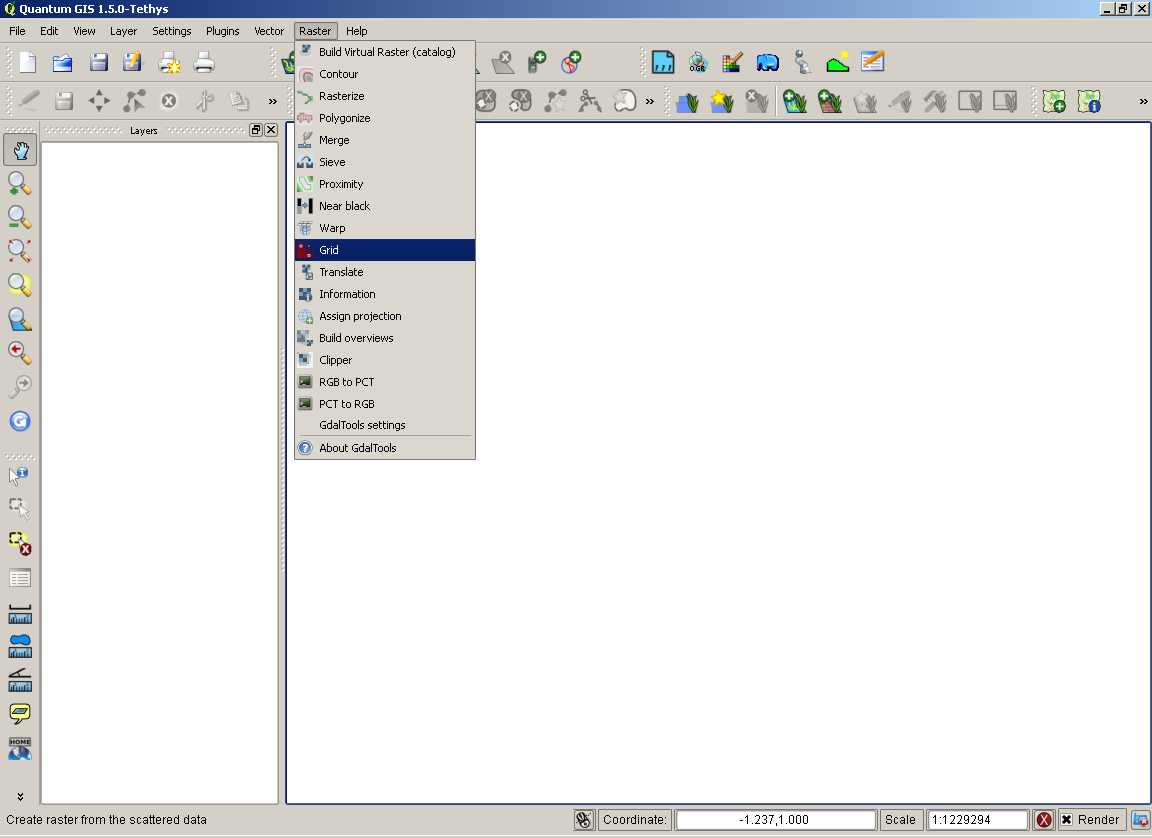
\includegraphics[clip=true, width=7cm]{plugins_gdaltools_images/raster_menu}
\end{figure}

\subsection{Exemples}\label{gdal_examples}
%Below are some examples of use of the tools.
%\subsubsection{Getting information about a raster}
Voici quelques exemples d'usage de ces outils.
\subsubsection{Obtenir des informations}
\begin{figure}[ht]
   \centering
%   \caption{\label{gdalinfo}The \emph{Information} dialog window \nixcaption}
   \caption{La fenêtre \emph{Information} \nixcaption}\label{gdalinfo}
   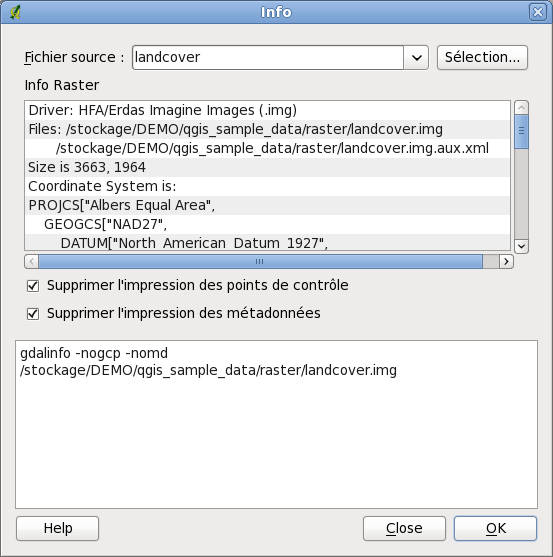
\includegraphics[clip=true, width=10cm]{plugins_gdaltools_images/gdalinfo}
\end{figure}

\subsubsection{Création de lignes de contours}
Cet exemple montre la création de lignes de contours à partir d'une tuile SRTM
\begin{figure}[ht]
   \centering
   \caption{La fenêtre \emph{Création de contours} \nixcaption}\label{gdal_contour}
   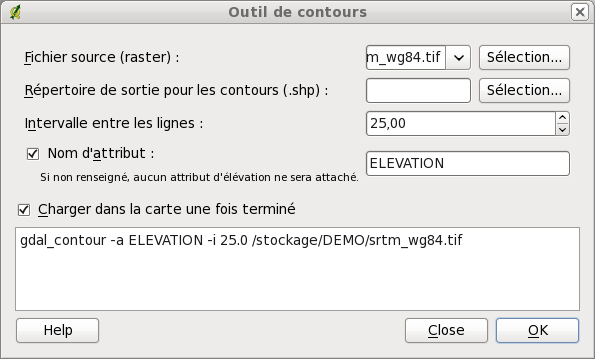
\includegraphics[clip=true, width=12cm]{plugins_gdaltools_images/gdal_contour}
\end{figure}
and the result:
\begin{figure}[ht]
   \centering
   \caption{La couche vectorielle résultante \nixcaption}\label{gdal_contour}
   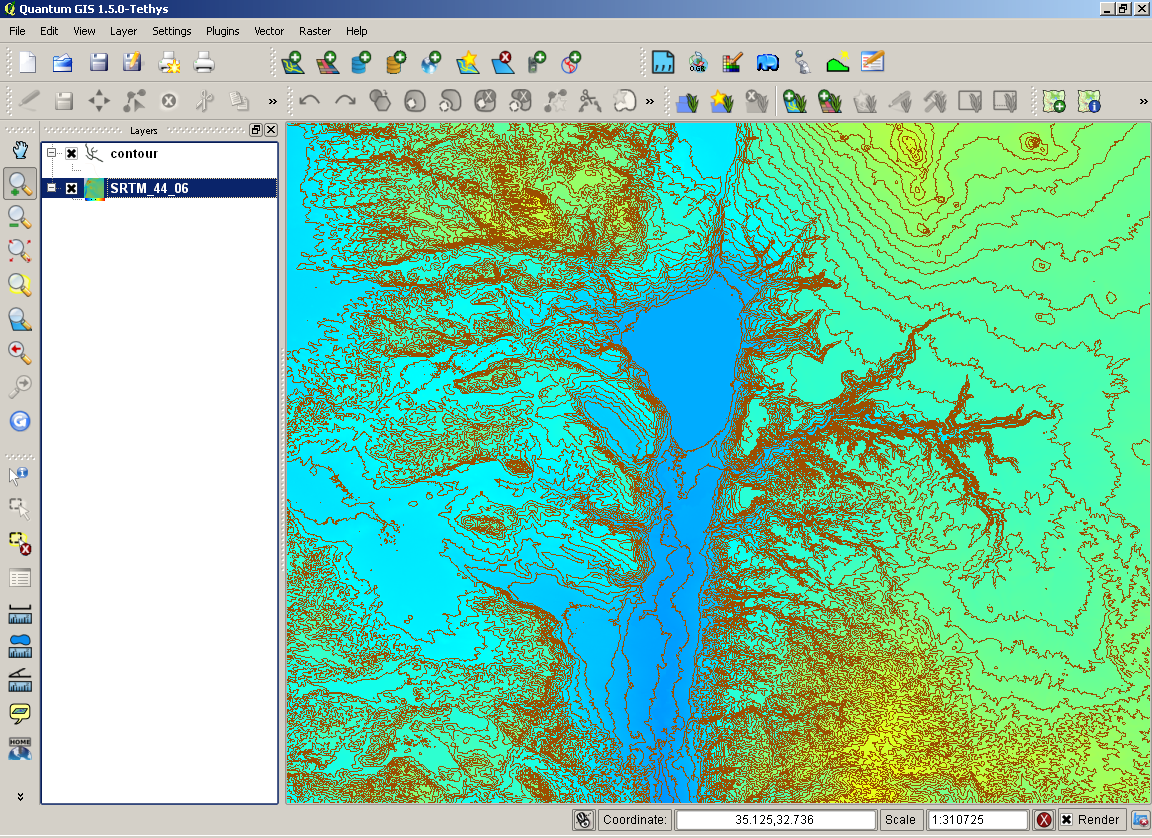
\includegraphics[clip=true, width=12cm]{plugins_gdaltools_images/qgis_contours}
\end{figure}

%\subsubsection{Using GDALwarp to reproject a raster}
%Here's the dialog window for reprojecting a landcover image, originally in the Albers Equal Area projection for Alaska (from the QGIS sample dataset) into Lon/Lat WGS84 (EPSG:4326).
\subsubsection{utiliser GDALwarp pour reprojeter un raster}
Voici la fenêtre permettant de reprojeter une image à l'origine en Albers Equal Area en Lon/Lat WGS84 (EPSG:4326).
\begin{figure}[ht]
   \centering
   \caption{\label{gdalwarp} La fenêtre \emph{Projection}\nixcaption}
   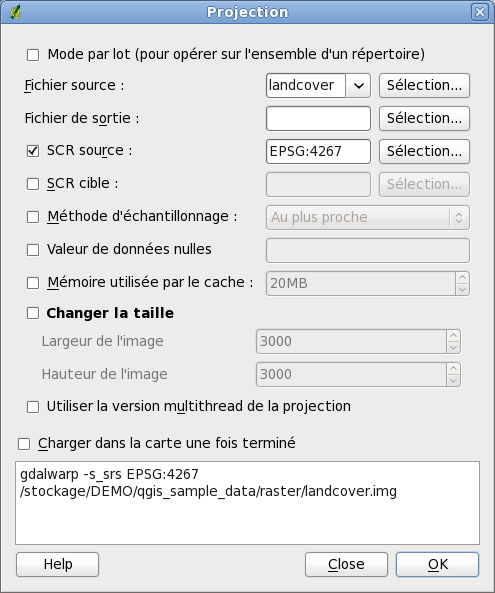
\includegraphics[clip=true, width=10cm]{plugins_gdaltools_images/gdalwarp}
\end{figure}

\FloatBarrier
